\documentclass[fleqn]{article}
\usepackage[utf8]{inputenc}
\usepackage{fullpage}
\usepackage[english]{babel}
\usepackage[pdftex]{graphicx}
\usepackage{float}
\usepackage{subcaption}
\usepackage{todonotes}
\usepackage{amsmath}
\usepackage{spverbatim}
\usepackage{longtable}
\usepackage{placeins}
\usepackage{color, colortbl}
\usepackage{csquotes}
\usepackage{framed}
\usepackage{listings}
\newcommand{\HRule}{\rule{\linewidth}{0.5mm}}

\begin{document}

\begin{titlepage}

\begin{center}


% Upper part of the page

\includegraphics[width=0.5\textwidth]{epl-logo.png}\\[1cm]

\textsc{\LARGE catholic university of louvain-la-neuve}\\[1.5cm]

\textsc{\Large INGI2143 - Concurrent Systems}\\[0.5cm]


% Title
\HRule \\[0.4cm]
{ \huge \bfseries Report - Assignment 3}\\[0.4cm]

\HRule \\[1.5cm]

% Author

{\huge Alexandre \textsc{Hauet} \\[0.6cm] Florian \textsc{Thuin}}


\vfill

% Bottom of the page
{\large \today}

\end{center}

\end{titlepage}

% Graphical representation of the Petri Net
\section{Graphical display of the Petri Nets}
\label{sec:Graphical display of the Petri Nets}
\begin{figure}[!h]
  \centering
    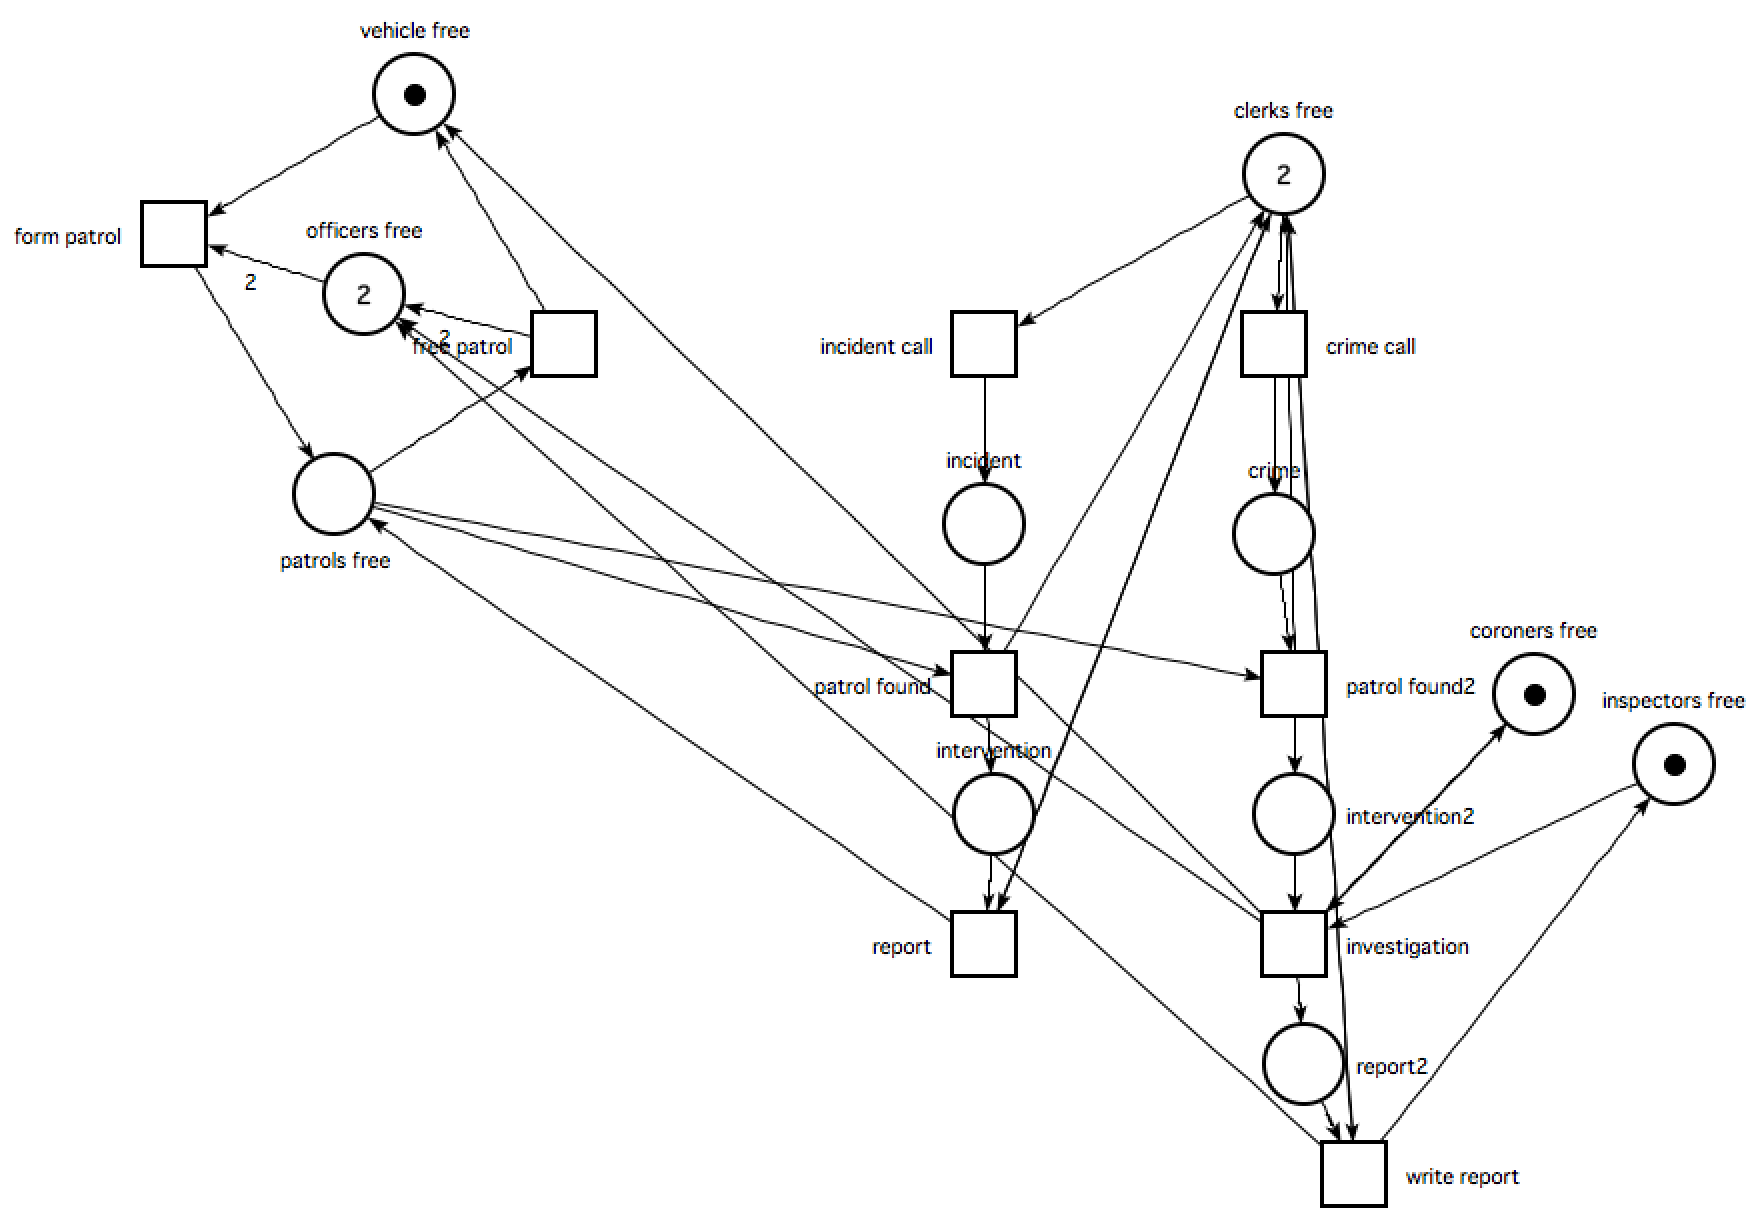
\includegraphics[width=\textwidth]{model.png}
    \caption{Picture of the Petri Net model}
\end{figure}


% T- and P-invariants
\section{T- and P-invariants}
\label{sec:T- and P-invariants}

\subsection{P-Semi-Flows}

\begin{lstlisting}
{coroners free}
{clerks free} crime incident
{inspectors free} {report on crime}
{intervention on incident place}*2 {intervention on crime place}*2 {officers free} {patrols free}*2 {report on crime}
{intervention on incident place} {intervention on crime place} {patrols free} {vehicle free}
\end{lstlisting}

These invariants show how parts of the Petri net are related in terms of amount
of tokens. It is the result of a set of linear \enquote{flow} equations from the
incidence matrix. \newline

For example, \verb#{coroners free}# place always have the same amount of tokens
(because the arrow leaves this place to a transition that has an arrow to this
place). \newline

Another example is that the amount of tokens in \verb#{clerks free}# and
\verb#crime# and \verb#incident# is always the same. It can be explained by the
fact that the arrows from \verb#{clerks free}# leaves weither to \verb#crime#
or to \verb#incident#, which next transitions lead to send the token back to
\verb#{clerks free}#. \newline

The third one is \verb#{inspectors free}# and \verb#{report on crime}# that will always
have the same amount of tokens because the transition coming to
\verb#inspectors free# needs one token from \verb#{report on crime}# that needs a token
from the \verb#inspectors free#. So if one or more tokens exist, they will
always loop between those two places and nothing is ever lost or ever
duplicate. \newline

The fourth one and fifth one are much longer but follow the exact same logic.
If you sum the number of tokens in each place of a P-semi-flow, it will always
be the same, no matter which set of transitions you choose. \newline

\subsection{T-Semi-Flows}

\begin{lstlisting}
{incident call} {patrol found} {report on incident}
{crime call} {form patrol} investigation {patrol found for crime} {write the report}
{form patrol} {free patrol}
\end{lstlisting}

These invariants show how the Petri can get back to the exact same state. \newline

Activating a transition \verb#{incident call}#, then a \verb#{patrol found}#
transition, then a \verb#{report on incident}# transition will take the Petri
net in the exact same state it was before. \newline

The same goes for the two other T-semi-flows, if you execute them as a loop,
you will come back to the exact same Petri Net state (with the same amount of
token everywhere). \newline


% Reachability analysis
\section{Reachability analysis}
\label{sec:Reachability analysis}
Our model is bounded, because as we can see in P-invariant and T-invariant there
 are no creation of new tokens. Compared to the inital state, they are no
 multiplication of the number of clerks, officers, vehicles, inspectors and
 coroners.


\begin{table}[h]
   \begin{tabular}{|r|r|}
       \hline
       Number of states & 30 \\
       \hline
       Number of transitions & 60 \\
       \hline
       Number of deadlock states & 6 \\
       \hline
   \end{tabular}
\end{table}


% Deadlock trace
\section{Deadlock trace}
\label{sec:Deadlock trace}


% Petri Net variant
\section{A variant of the Petri Net}
\label{sec:A variant of the Petri Net}
The places that have unbounded markings in the graph are ''incident call'' and ''crime call''. Because now when the clercks receive a call for a crime or a incident, they don't need  to wait for a patrol in order to handle the situation. They can receive directly a other call.


\end{document}
